\documentclass[tikz,border=2pt]{standalone}
\begin{document}
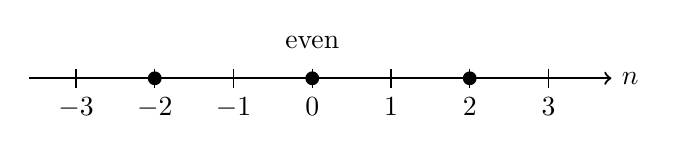
\begin{tikzpicture}[x=1cm]
  \draw[->, thick] (-3.6,0) -- (3.8,0) node[right] {$n$};
  \foreach \n in {-3,...,3} {
    \draw (\n,0.12) -- (\n,-0.12) node[below] {$\n$};
  }
  \foreach \n in {-2,0,2} {
    \fill (\n,0) circle (2.5pt);
  }
  \node[above] at (0,0.25) {even};
\end{tikzpicture}
\end{document}
